\section{Seed distributions and the step model}\label{sec:18.3}

At $\omega = \SI{5}{eV}$ in silicon the step model of \cref{eq:1.5-step} puts every event in the two-pair bin. The cascade of \cref{sec:18.1}, with the constant calibrated in \cref{sec:18.4}, puts two pairs in \SI{17}{\percent} of the events started by a dark-matter kick at $q_0 = \alpha m_e$ and one pair in the rest. A search with a two-pair threshold therefore records about one in six of the \SI{5}{eV} events that the step model predicts. The cascade differs from the step model in two respects: how the \SI{3.84}{eV} above the gap is shared between the electron and the hole, and how often each carrier emits a phonon instead of ionizing at a few eV. The energy sharing and the phonon emission both enter through the hand-off \cref{eq:8.7-cond}. Once a final-state class has been turned into the energies of its two carriers, the generating function of \cref{sec:18.1} yields the whole pair-number distribution. The step model and a cascade seeded by a fixed split of the energy are limits of the pair-number distribution that replace the seed by a rule, and they fail in the few-pair bins, where the rule matters most.

\subsection{The seed distribution}\label{sec:18.3-seed}

A final-state class $\Lambda$ of the zero-phonon pair sector puts an electron at $E_{\mathrm{e}}(\Lambda)$ above the conduction minimum and a hole at $E_{\mathrm{h}}(\Lambda)$ below the valence maximum, with $E_{\mathrm{e}} + E_{\mathrm{h}} = \omega - \Eg$. In the energy-only reduction of \cref{sec:18.1-reductions} the cascade of the pair depends on these two energies; the crystal momenta $\vect{k} + \vect{q}$ and $\vect{k}$ matter only for the first collisions. Keeping the energies and dropping the momenta loses the first-generation memory that \cref{sec:18.1-reductions} locates. The input from the dark-matter interaction is then a distribution of carrier energies. The \emph{seed distribution} at momentum transfer $\vect{q}$, energy $\omega$ and velocity $\vect{v}$ is
\begin{equation}
  P_{\mathrm{seed}}(E_{\mathrm{e}},E_{\mathrm{h}}|\vect{q},\omega,\vect{v}) = \frac{\sum_\Lambda\sum_{a,b}\mathfrak{D}_{ab}(\vect{q},\vect{v})\,S_{ab}(\vect{q},\omega;\Lambda)\,\delta\bigl(E_{\mathrm{e}} - E_{\mathrm{e}}(\Lambda)\bigr)\,\delta\bigl(E_{\mathrm{h}} - E_{\mathrm{h}}(\Lambda)\bigr)}{\sum_{a,b}\mathfrak{D}_{ab}(\vect{q},\vect{v})\,S_{ab}(\vect{q},\omega)} ,
  \label{eq:18.3-seed}
\end{equation}
the probability density that the interaction leaves the electron at $E_{\mathrm{e}}$ and the hole at $E_{\mathrm{h}}$. The class-resolved responses add up to $S_{ab}(\vect{q},\omega)$ by \cref{eq:8.7-resolved}, so $P_{\mathrm{seed}}$ integrates to one when every class at $(\vect{q},\omega)$ is a pair, and to the pair share of the response otherwise; the other sectors seed their own cascades. A pair made together with a phonon of energy $\omega_{\vect{Q}}$ has $E_{\mathrm{e}} + E_{\mathrm{h}} = \omega - \omega_{\vect{Q}} - \Eg$, and the phonon energy goes to heat once (\cref{sec:8.7}). With one coupling row the seed distribution is independent of $\vect{v}$ and of the dark-matter model, as the class weights of \cref{sec:8.7-handoff} are; with several rows it depends on both. In the zero-phonon sector energy conservation leaves one variable, the electron's share $f_{\mathrm{e}} = E_{\mathrm{e}}/(\omega - \Eg)$ of the energy above the gap.

The generating function of \cref{eq:18.1-seed} turns the seed into a pair number. Keep only the pair-number variable, $s = \ee^{\lambda_N}$, and let $\mathfrak{G}_t(x;s)$ be the energy-only solution of \cref{eq:18.1-backward}: the generating function of the number of ionizations that a carrier of type $t$ at kinetic energy $x$ makes in its subtree. The seed pair is counted by the factor $s$, and the two subtrees are independent, so the cascade distribution of a class is the coefficient
\begin{equation}
  P_{\mathrm{casc}}(N_{\mathrm{eh}}|\Lambda) = [s^{N_{\mathrm{eh}}}]\;s\,\mathfrak{G}_{\mathrm{e}}\bigl(E_{\mathrm{e}}(\Lambda);s\bigr)\,\mathfrak{G}_{\mathrm{h}}\bigl(E_{\mathrm{h}}(\Lambda);s\bigr) ,
  \label{eq:18.3-pcasc}
\end{equation}
where $[s^n]$ takes the coefficient of $s^n$. The cascade distribution depends on $\Lambda$ only through the two carrier energies. Write $P_{\mathrm{casc}}(N_{\mathrm{eh}}|\Lambda)$ as $\int\dd E_{\mathrm{e}}\,\dd E_{\mathrm{h}}\,\delta(E_{\mathrm{e}} - E_{\mathrm{e}}(\Lambda))\,\delta(E_{\mathrm{h}} - E_{\mathrm{h}}(\Lambda))\,P_{\mathrm{casc}}(N_{\mathrm{eh}}|E_{\mathrm{e}},E_{\mathrm{h}})$ inside the class sum of \cref{eq:8.7-cond}, and exchange the sum with the integral. The class sum then becomes the numerator of \cref{eq:18.3-seed}:
\begin{equation}
  P(N_{\mathrm{eh}}|\vect{q},\omega,\vect{v}) = \int\dd E_{\mathrm{e}}\,\dd E_{\mathrm{h}}\;P_{\mathrm{seed}}(E_{\mathrm{e}},E_{\mathrm{h}}|\vect{q},\omega,\vect{v})\;P_{\mathrm{casc}}(N_{\mathrm{eh}}|E_{\mathrm{e}},E_{\mathrm{h}}) .
  \label{eq:18.3-pq}
\end{equation}
The generating function of \cref{eq:18.3-pq} is $s\int P_{\mathrm{seed}}\,\mathfrak{G}_{\mathrm{e}}\mathfrak{G}_{\mathrm{h}}$, a power series with nonnegative coefficients that converges on $|s| \le 1$. The discrete Fourier sum \cref{eq:E.24-dft} of this generating function at $N_z$ roots of unity returns $\sum_jP(N_{\mathrm{eh}} + jN_z)$, the exact probability once $N_z$ exceeds every pair number with appreciable weight.

The backward recursion alone guarantees three things: the pair-number distribution is normalized, it is exactly one pair below $(1 + \theta_{\mathrm{ii}})\Eg$, and its variance splits into a cascade part and a seed part. First, each $\mathfrak{G}_t$ is a probability generating function, because the recursion of \cref{eq:18.1-backward} maps products and mixtures of generating functions to generating functions; \cref{eq:18.3-pq} is then normalized and nonnegative. Second, below $\theta_{\mathrm{ii}}\Eg$ no carrier ionizes, $\mathfrak{G}_t = 1$, and $P_{\mathrm{casc}} = \delta_{N_{\mathrm{eh}}1}$ exactly. The first ionization becomes possible at $\omega = (1 + \theta_{\mathrm{ii}})\Eg$, which is \SI{2.32}{eV} in silicon with $\theta_{\mathrm{ii}} = 1$, for a seed that gives all the energy to one carrier. Third, the moments separate the cascade from the seed. Let $m_t(x)$ and $v_t(x)$ be the mean and variance of the number of ionizations in one subtree, and let $\langle\cdot\rangle_{\mathrm{seed}}$ average over $P_{\mathrm{seed}}$. The law of total variance gives
\begin{equation}
  \langle N_{\mathrm{eh}}\rangle = 1 + \bigl\langle m_{\mathrm{e}}(E_{\mathrm{e}}) + m_{\mathrm{h}}(E_{\mathrm{h}})\bigr\rangle_{\mathrm{seed}} , \qquad
  \operatorname{Var}N_{\mathrm{eh}} = \bigl\langle v_{\mathrm{e}} + v_{\mathrm{h}}\bigr\rangle_{\mathrm{seed}} + \operatorname{Var}_{\mathrm{seed}}\bigl(m_{\mathrm{e}} + m_{\mathrm{h}}\bigr) .
  \label{eq:18.3-moments}
\end{equation}
The second term of the variance is the spread of the subtree means over the seed. It vanishes when $m_{\mathrm{e}} + m_{\mathrm{h}}$ takes one value on the whole support of the seed, for a single split and in the forced region $\omega < (1 + \theta_{\mathrm{ii}})\Eg$, where both means are zero.

$P_{\mathrm{seed}}$ is the per-pair weight of \cref{eq:8.7-IP} or of the screened form \cref{eq:8.7-screened}, binned in the two carrier energies; a library of computed responses stores $P_{\mathrm{seed}}$ in this binned form. With the functions $\mathfrak{G}_t$ tabulated on an energy grid, the seeded distribution costs one integral per momentum transfer, energy and pair of coupling rows.

\subsection{Pair-number distributions in silicon}\label{sec:18.3-silicon}

\Cref{fig:18-pn10} shows \cref{eq:18.3-pq} at $\omega = \SI{10}{eV}$ for six seeds run through one cascade. The cascade is the random-$k$ model of \cref{sec:18.1-reductions} with the silicon parameters of \cref{sec:18.2-heat}. The dark-matter seed comes from the empirical-pseudopotential bands of \cref{we:8-pairs}: the pair weights of the density at $\vect{q}_0 = \alpha m_e\hat{\vect{x}}$, without screening. The photon seed is the optical limit of the same bands. The model bands have a gap of \SI{0.82}{eV}, so each band seed is taken at the same excess energy $\omega - \Eg$ as the cascade uses. To compare two pair-number distributions we use the total-variation distance $d_{\mathrm{TV}}(P,Q) = \tfrac12\sum_N|P(N) - Q(N)|$, which is the largest difference between the probabilities that the two distributions assign to any set of pair numbers, for instance to the events above a search threshold. Screening hardly moves the energy shares: at \SI{10}{eV} the screened out-state seed of \cref{we:8-pairs} and its unscreened counterpart give distributions with $d_{\mathrm{TV}} = 0.010$.

\begin{figure}[tbp]
  \centering
  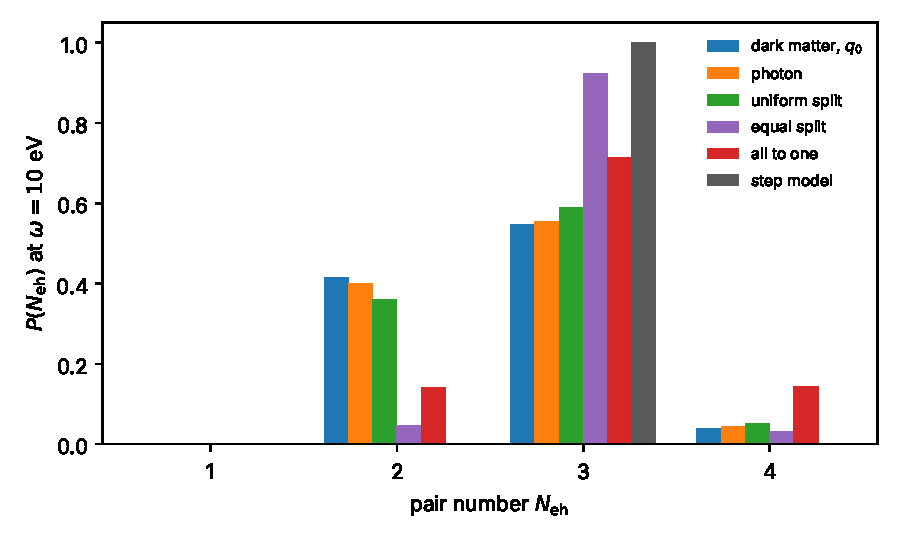
\includegraphics[width=0.85\linewidth]{figures/ch18/fig18_3.pdf}
  \caption{Pair-number distribution $P(N_{\mathrm{eh}})$ at $\omega = \SI{10}{eV}$ in silicon, \cref{eq:18.3-pq}, for six seeds in one cascade: the energy-only random-$k$ model of \cref{sec:18.1-reductions} with $\Eg = \SI{1.160}{eV}$, $\omega_{\mathrm{AB}} = \SI{63}{meV}$, $\theta_{\mathrm{ii}} = 1$, holes below \SI{12}{eV} and $A_{\mathrm{AB}} = \SI{5.703}{eV^3}$, calibrated to $\varepsilon_{\mathrm{eh}} = \SI{3.749}{eV}$. The band seeds are a dark-matter kick at $q_0 = \alpha m_e$ along [100] (independent-particle pair weights of the density, empirical-pseudopotential bands of \cref{we:8-pairs}) and an absorbed photon (optical limit of the same bands). The other four seeds are the fixed splits of \cref{sec:18.3-limits} (uniform, equal, and all the energy to one carrier) and the step model \cref{eq:1.5-step} with $\varepsilon_{\mathrm{eh}} = \SI{3.749}{eV}$. Band seeds are used at the excess energy $\omega - \Eg$ of the model bands, whose gap is \SI{0.82}{eV}. Means: 2.626 (dark matter), 2.645 (photon), 2.691, 2.985 and 3.003 (the three splits), 3 (step model). $P(1)$ and $P(5)$ are below 0.002 for every seed. Probabilities from the generating function at $N_z = 32$ roots of unity; no distribution in this section has a mean above six.}
  \label{fig:18-pn10}
\end{figure}

The dark-matter seed yields two pairs with probability 0.414, three with 0.547 and four with 0.039. The mean, 2.626 pairs, corresponds to \SI{3.81}{eV} per pair, \SI{1.6}{\percent} above the high-energy pair energy. The photon seed yields 0.400, 0.555 and 0.045, and its mean is 2.645. The step model puts every event in the three-pair bin; it overstates the mean by \SI{14}{\percent} and misses the two-pair bin entirely. Of the three splits of \cref{sec:18.1-seed}, the equal split puts three pairs in \SI{92}{\percent} of events, the uniform split behaves like the band seeds, and giving everything to one carrier fills the four-pair bin with probability 0.143.

The variance shows where the seed enters. For the dark-matter seed \cref{eq:18.3-moments} splits $\operatorname{Var}N_{\mathrm{eh}} = 0.314$ into 0.283 from the subtrees and 0.031 from the spread of the seed. The equal split has no seed term, and its variance is 0.079, a quarter of the band-seed value. The subtree mean is far from linear in the share: at $f_{\mathrm{e}} = \tfrac14$, \SI{2.21}{eV} on one carrier and \SI{6.63}{eV} on the other, the two carriers make 2.436 pairs, against 2.985 at the equal split and 3.003 with all \SI{8.84}{eV} on one carrier. A carrier at \SI{2.21}{eV} almost never ionizes, while one at \SI{4.42}{eV} usually does once, so the count depends on how many carriers end up a little above \SI{4}{eV}.

\begin{workedexample}{The step model against the cascade at 5 eV}\label{we:18-step5}
Take $\omega = \SI{5}{eV}$ in silicon with the constants of \cref{fig:18-pn10}. The step model puts $N_{\mathrm{eh}} = 1 + \lfloor(5 - 1.160)/3.749\rfloor = 1 + \lfloor1.024\rfloor = 2$ pairs for every event; the literature values $\Eg = \SI{1.11}{eV}$ and $\varepsilon_{\mathrm{eh}} = \SI{3.6}{eV}$ of \cref{sec:1.5} give 2 as well.

In the cascade, the pair shares $\omega - \Eg = \SI{3.84}{eV}$. Consider first a seed that gives all of it to one carrier. Below $\Eg$ the carrier cannot ionize; above, the probability that its next collision is an ionization is $p_{\mathrm{ii}}(E) = [1 + \varGamma_{\mathrm{ph}}/\varGamma_{\mathrm{ii}}]^{-1}$ from \cref{eq:18.1-randomk}. The ionization probability is 0.0041 at \SI{2}{eV}, 0.0184 at \SI{2.5}{eV}, 0.049 at \SI{3}{eV}, 0.100 at \SI{3.5}{eV} and 0.145 at \SI{3.84}{eV}. As long as the carrier does not ionize, it walks down in steps of $\omega_{\mathrm{AB}}$: from \SI{3.84}{eV} it makes 43 collisions above $\Eg$. The probability that none of them is an ionization is
\begin{equation*}
  P_{\mathrm{no}} = \prod_{k=0}^{42}\bigl[1 - p_{\mathrm{ii}}(3.84\,\mathrm{eV} - k\,\omega_{\mathrm{AB}})\bigr] = 0.176 .
\end{equation*}
Replacing the sum of $-\ln(1 - p_{\mathrm{ii}}) \approx p_{\mathrm{ii}}/(1 - p_{\mathrm{ii}})$ over steps by an integral over energy, $\ln P_{\mathrm{no}} \approx -\omega_{\mathrm{AB}}^{-1}\int_{\Eg}^{3.84\,\mathrm{eV}}\dd E\;\varGamma_{\mathrm{ii}}/\varGamma_{\mathrm{ph}} = -1.735$, which leads to the same 0.176. If the carrier does ionize, the three products share at most $3.84 - 1.16 = \SI{2.68}{eV}$, and a second ionization follows with probability 0.002. This seed therefore leaves one pair with probability 0.176 and two with 0.822. A seed that splits the energy equally leaves two carriers at \SI{1.92}{eV}, each of which escapes ionization with probability 0.990, so that \SI{98}{\percent} of events end with one pair.

The dark-matter seed at $q_0$ lies between the one-sided seed and the equal split. At this energy the electron takes \SI{2.08}{eV} of the \SI{3.84}{eV} on average, and \SI{26}{\percent} of the weight has one carrier with more than three quarters of the energy. Averaging $P_{\mathrm{no}}(E_{\mathrm{e}})P_{\mathrm{no}}(E_{\mathrm{h}})$ over the seed in \cref{eq:18.3-pq} yields
\begin{equation*}
  P(1) = 0.831 , \qquad P(2) = 0.169 , \qquad P(3) = 6\times10^{-5} ,
\end{equation*}
a mean of 1.169 pairs and \SI{4.28}{eV} per pair. Above a two-pair threshold the step model therefore counts 5.9 times as many \SI{5}{eV} events as this cascade does; the full-band cascade of \cref{sec:18.3-fullband} raises the factor to about ten. The photon seed has $P(2) = 0.190$, \SI{12}{\percent} more than the dark-matter seed.
\end{workedexample}

\subsection{The full-band cascade as reference}\label{sec:18.3-fullband}

Every distribution so far comes from the energy-only cascade with its one constant fitted to the measured pair energy. A cascade with no fitted constant replaces the random-$k$ kernels by the kernels of \cref{sec:18.1} on full bands, in the standard full-band Monte Carlo form~\cite{fischetti1988monte}. In the calculation we use as reference, the bands are the empirical pseudopotential bands of Cohen and Bergstresser~\cite{cohen1966band}, with the form factors refit to measured transition energies; impact ionization is the golden rule with the diagonal, statically screened Coulomb kernel~\cite{cappellini1993model}, its direct and exchange terms combined as in Kane's form quoted by Kotani and van Schilfgaarde~\cite[Eq.~(5)]{kotani2010impact}; and phonon emission uses the deformation potentials and phonon energies of Refs.~\cite{lundstrom2000fundamentals,jacoboni1983monte}, \cite[Table~III]{li2021deformation}; the gap is $\Eg = \SI{1.160}{eV}$. The seeds are the pairs a dark-matter particle with a heavy mediator leaves in the same bands, with their crystal momenta. The calculation is varied jointly over the screening (static and dynamic), the phonon couplings (these values against first-principles ones, which weigh electron losses by 0.52 and hole losses by 3.0) and the exchange factor near threshold (0.5 to 1.0), and the ranges below are the envelope of these variants, for pair probabilities with the error of the $\vect{k}$ grid added.

At \SI{5}{eV} the full-band cascade puts two or more pairs in a fraction $0.097$ of the dark-matter events, with the envelope $[0.030, 0.173]$, against the 0.169 of the energy-only cascade in \cref{we:18-step5}. The step model, which puts every event in the two-pair bin, then overcounts that bin about tenfold, and at least sixfold anywhere in the envelope; the thirtyfold end of the envelope comes from one extreme corner alone, static screening of the weaker kind with tripled hole couplings and the lowest exchange factor. The energy-only cascade remains the working model of this chapter, because it is calibrated and fast. Recalibrated to the pair energy of each full-band variant, so that only the shape of the kernels differs, the energy-only cascade lies 0.12 to 0.20 in $d_{\mathrm{TV}}$ from the full-band distribution between 6 and \SI{8}{eV}. The soft onset of impact ionization near threshold matters most in this range, and the distance grows with the pair energy of the variant. On the same footing the uniform split lies 0.11 to 0.12 away, the equal split 0.45 to 0.50 and the step model 0.79 to 0.83.

\subsection{Fixed splits and the step limit}\label{sec:18.3-limits}

A fixed split replaces the seed distribution of \cref{eq:18.3-pq} by a distribution of the electron's share $f_{\mathrm{e}}$ that is the same for every process at a given $\omega$ and symmetric under the exchange of electron and hole. Three fixed splits bracket the range: all the energy on one carrier, a uniform share, and the equal split. The constant term $b_N$ of the mean (\cref{sec:18.2-heat}) depends on the seed. In the cascade of \cref{fig:18-pn10}, with $\omega/\varepsilon_{\mathrm{eh}}$ subtracted at the pair energy of the same calculation, it is 0.008 for the uniform split and 0.35 for a seed that gives all the energy to one carrier.

The step model is the limit in which every pair has a fixed cost. Let the first pair cost $\Eg$ and every further one exactly $\varepsilon_{\mathrm{eh}}$. The energy $\omega - \Eg$ left after the first pair is then spent by a renewal chain with the deterministic loss $\varepsilon_{\mathrm{eh}}$, which fits $\lfloor(\omega - \Eg)/\varepsilon_{\mathrm{eh}}\rfloor$ losses (\cref{app:C.11}). The pair number is
\begin{equation}
  N_{\mathrm{eh}}^{\mathrm{step}}(\omega) = 1 + \left\lfloor\frac{\omega - \Eg}{\varepsilon_{\mathrm{eh}}}\right\rfloor , \qquad P_{\mathrm{casc}}(N_{\mathrm{eh}}|\Lambda) = \delta_{N_{\mathrm{eh}},N_{\mathrm{eh}}^{\mathrm{step}}(\omega)} ,
  \label{eq:18.3-step}
\end{equation}
which is \cref{eq:1.5-step}, with a Fano factor of zero. Both the seed and the competition with phonons have been replaced by one cost per pair. In the forced region, $\omega < (1 + \theta_{\mathrm{ii}})\Eg$, the step model is exact. Above the forced region, even the mean is wrong. Over one period of $\omega$ the floor function loses $\tfrac12$ on average (\cref{app:C.11}), so the step model has the mean $(\omega - \Eg)/\varepsilon_{\mathrm{eh}} + \tfrac12 = \omega/\varepsilon_{\mathrm{eh}} + 0.19$ in silicon, against $\omega/\varepsilon_{\mathrm{eh}} + b_N$ in the cascade, with $b_N$ between 0.008 and 0.35 depending on the seed. This error in the mean falls as $1/\langle N_{\mathrm{eh}}\rangle$. The step-model distribution itself never approaches the cascade distribution. For a single bin $n$ the distance $d_{\mathrm{TV}}$ is $1 - P(n)$. The cascade distribution spreads over a width $\sigma_N = (F_{\mathrm{eh}}\omega/\varepsilon_{\mathrm{eh}})^{1/2}$ that grows with $\omega$: at \SI{20.2}{eV} the computed distribution of the dark-matter seed has $\sigma_N = 0.79$ and its largest bin holds 0.45, so the step model misplaces more than half of the events there, and the misplaced fraction grows with the width.

\Cref{lim:18.3a} compares each phenomenological seed with the dark-matter seed from the gap to \SI{21}{eV}, the range of the few-pair bins in silicon.

\begin{limitbox}[Step model and fixed splits][lim:18.3a]
The step model is \cref{eq:18.3-step}~\cite[Eq.~(5.1)]{essig2016direct}; the three fixed splits above are each run through the cascade by \cref{eq:18.3-pcasc}.
\par\smallskip
{\centering
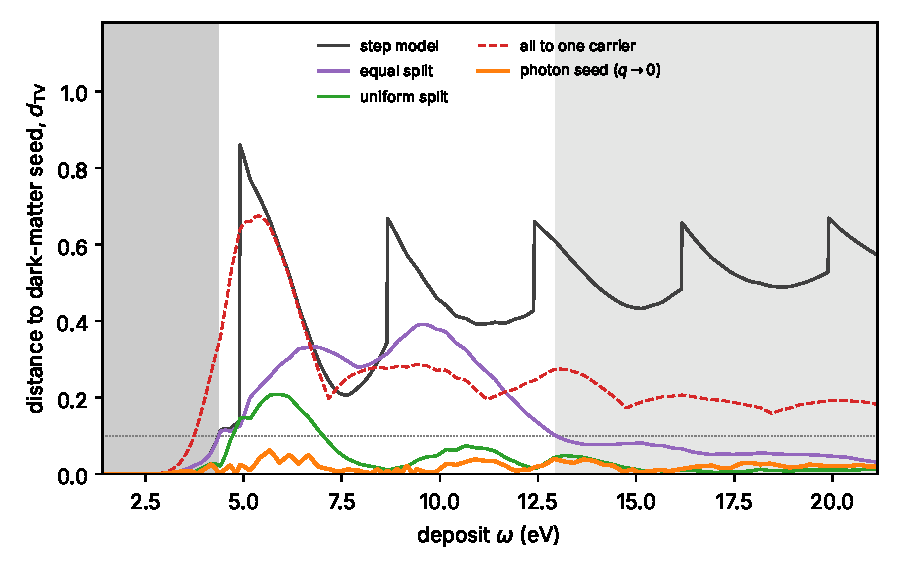
\includegraphics[width=\linewidth]{figures/ch18/limit18_3a.pdf}
\captionof{figure}{Distance $d_{\mathrm{TV}}$ between the pair-number distribution of each phenomenological seed and the distribution of the dark-matter seed at $q_0 = \alpha m_e$ along [100], against the deposit $\omega$ in silicon. All seeds run through one cascade, the energy-only random-$k$ model of \cref{sec:18.1-reductions} with $\Eg = \SI{1.160}{eV}$, $\omega_{\mathrm{AB}} = \SI{63}{meV}$, $\theta_{\mathrm{ii}} = 1$, holes below \SI{12}{eV} and $A_{\mathrm{AB}} = \SI{5.703}{eV^3}$. Black: step model, $\varepsilon_{\mathrm{eh}} = \SI{3.749}{eV}$. Purple, green and red dashed: the equal split, the uniform split and all the energy to one carrier, with the seeds that put a hole above \SI{12}{eV} removed. Orange: the photon ($q \to 0$) seed of the same empirical-pseudopotential bands as the dark-matter seed. Band seeds are computed every \SI{0.25}{eV} of the excess energy $\omega - \Eg$ (model gap \SI{0.82}{eV}) and interpolated linearly; the curves use a \SI{0.02}{eV} grid. Dark gray: $\omega < \SI{4.37}{eV}$, where the step model and the uniform and equal splits are within 0.1 of the dark-matter seed. Light gray: $\omega > \SI{12.95}{eV}$, where the uniform and equal splits are again within 0.1 of the dark-matter seed. Dotted: $d_{\mathrm{TV}} = 0.1$.}\label{fig:18-limit-seed}
\par}
\smallskip
Between \SI{4.4}{eV} and \SI{13}{eV} the split of the energy decides the count, so the split must come from the bands and the operator that made the pair. There the uniform and equal splits reach distances of 0.21 and 0.39, the one-sided split 0.67, and the step model is off by up to 0.86 at its first step, $\omega = \Eg + \varepsilon_{\mathrm{eh}} = \SI{4.91}{eV}$.
\end{limitbox}

Below \SI{4.37}{eV} the step model and the fixed splits hold because few carriers ionize: the dark-matter seed leaves one pair with probability above 0.9, and so does any split that avoids putting the whole energy on one carrier. The distance of the step model exceeds 0.1 from \SI{4.37}{eV} on: at its first step the step model moves every event into the two-pair bin while the cascade puts 0.14 there, and its distance stays above 0.2 up to \SI{21}{eV}, above 0.39 beyond \SI{9}{eV}. The uniform and equal splits come within 0.04 of the dark-matter seed at \SI{21}{eV}. The one-sided split stays 0.18 away even there. At \SI{21}{eV} the valence band no longer holds the whole energy, so this split can put the energy only on the electron, and its mean lies 0.36 pairs above the mean of the dark-matter seed. A shift of the mean by a fixed amount gives a distance that decreases only as $\sigma_N^{-1} \propto \omega^{-1/2}$.

The photon seed is the case that matters in practice, because a photon calibration measures it, and the difference between the photon seed and the dark-matter seed is the error that \cref{sec:8.7-handoff} left open. In the energy-only cascade, with both seeds from the same band calculation on one $\vect{k}$ grid, the photon seed stays within 0.062 of the dark-matter seed everywhere, with the largest distance at \SI{5.67}{eV}, where the means differ by \SI{4.6}{\percent}. At \SI{10}{eV} the distance is 0.014, and above \SI{15}{eV} it is at most 0.03. These distances are internal to the energy-only model. They measure only the difference of the energy shares and carry the error of the photon seed's $\vect{k}$ grid: in the full-band calculation of \cref{sec:18.3-fullband} the photon seed moves by 0.11 to 0.14 between grids, as much as its distance from the dark-matter seed, so the full-band value of this distance is unresolved. The energy-only reduction drops the valleys and crystal momenta of the first generation, which the dark matter populates differently from a photon; a calculation that keeps the valleys and crystal momenta would add their share of the error. Absorption of a dark photon has no error from substituting the photon seed, because the absorbed dark photon leaves the same seed as a photon (\cref{sec:8.7-handoff}).

\subsection{Pair number at the readout}\label{sec:18.3-observable}

Every distribution so far is the distribution of the pair number at the end of the prompt cascade, about a picosecond after the deposit, when every carrier has reached its band edge. A detector reads the event microseconds to seconds later, and what it reads depends on more than the pair number. The induced charge depends on where the pairs are and how far each carrier drifts. Capture costs one gap per captured electron, and excitons change the measured Fano factor (\cref{sec:18.5}). A phonon readout records the heat with its spectrum. The cascade therefore records, besides $N_{\mathrm{eh}}$, further quantities $\mathfrak{m}$: the positions of the carriers at the end of the prompt cascade, the electron and hole counts separately, the spectrum of the emitted phonons and the energy stored in defects. Let $P_{\mathrm{det}}(\mathsf{R}|N_{\mathrm{eh}},\mathfrak{m})$ be the probability that the readout records $\mathsf{R}$, a charge, a phonon energy or both, at the time it reads. The distribution of the recorded quantity for an event of class $\Lambda$ is
\begin{equation}
  P_{\mathrm{obs}}(\mathsf{R}|\Lambda) = \sum_{N_{\mathrm{eh}}}\int\dd\mathfrak{m}\;P_{\mathrm{casc}}(N_{\mathrm{eh}},\mathfrak{m}|\Lambda)\;P_{\mathrm{det}}(\mathsf{R}|N_{\mathrm{eh}},\mathfrak{m}) ,
  \label{eq:18.3-obs}
\end{equation}
and it replaces $P_{\mathrm{casc}}$ in \cref{eq:8.7-handoff} when the rate is written for the recorded quantity. The quantities $\mathfrak{m}$ are read off the same cascade sample as the pair number, so the generating function of \cref{eq:18.1-backward} carries them as further components of the deposit.

The step model and \cref{eq:18.3-pq} are statements about one marginal of \cref{eq:18.3-obs}: the pair number at the end of the prompt cascade, with $P_{\mathrm{det}} = \delta_{\mathsf{R}N_{\mathrm{eh}}}$. Every later process acts on that marginal and on $\mathfrak{m}$ together. If each pair is collected independently with probability $f_{\mathrm{det}}$, the recorded number is thinned binomially, its Fano factor is $f_{\mathrm{det}}F_{\mathrm{eh}} + 1 - f_{\mathrm{det}}$ by \cref{eq:C.11-thinfano}, and $\mathfrak{m}$ drops out. If collection depends on position or on the carrier type, $\mathfrak{m}$ does not drop out, and the rate needs the joint law. \Cref{sec:18.5} treats the second factor of \cref{eq:18.3-obs} up to the end of the cascade; the readout itself is the subject of \cref{chap:20}.
